%%%%%%%%%%%%%%%%%%%%%%%%%%%%%%%%%%%%%%%%%
% fphw Assignment
% LaTeX Template
% Version 1.0 (27/04/2019)
%
% This template originates from:
% https://www.LaTeXTemplates.com
%
% Authors:
% Class by Felipe Portales-Oliva (f.portales.oliva@gmail.com) with template 
% content and modifications by Vel (vel@LaTeXTemplates.com)
%
% Template (this file) License:
% CC BY-NC-SA 3.0 (http://creativecommons.org/licenses/by-nc-sa/3.0/)
%
%%%%%%%%%%%%%%%%%%%%%%%%%%%%%%%%%%%%%%%%%

%----------------------------------------------------------------------------------------
%	PACKAGES AND OTHER DOCUMENT CONFIGURATIONS
%----------------------------------------------------------------------------------------

\documentclass[
	12pt, % Default font size, values between 10pt-12pt are allowed
	%letterpaper, % Uncomment for US letter paper size
	%spanish, % Uncomment for Spanish
]{fphw}

% Template-specific packages
\usepackage[utf8]{inputenc} % Required for inputting international characters
\usepackage[T1]{fontenc} % Output font encoding for international characters
\usepackage{multicol, latexsym, amsmath, amssymb}
\usepackage{blindtext}
\usepackage{subcaption}
\usepackage{caption}
\usepackage{wrapfig}
\usepackage{tabu}
\usepackage[dvipsnames]{xcolor}
\usepackage{floatflt}

\usepackage{graphicx} % Required for including images

\usepackage{booktabs} % Required for better horizontal rules in tables

\usepackage{listings} % Required for insertion of code

\usepackage{enumerate} % To modify the enumerate environment


%----------------------------------------------------------------------------------------
%	ASSIGNMENT INFORMATION
%----------------------------------------------------------------------------------------

\title{Assignment 2} % Assignment title

\author{Giuliano Martinelli 1915652, Gabriele Giannotta 1909375, Mario Dhimitri 1910181 } % Student name

\date{November 19th, 2020} % Due date

\institute{Sapienza Università di Roma \\ Data Science} % Institute 

\class{Advanced Machine Learning} % Course or class name

\professor{Fabio Galasso} % Professor 

%----------------------------------------------------------------------------------------

\begin{document}

\maketitle % Output the assignment title, created automatically using the information in the custom commands above

%----------------------------------------------------------------------------------------
%	ASSIGNMENT CONTENT
%----------------------------------------------------------------------------------------

\section*{Question 2 - Backpropagation}
\section* {2. a}

Verify that the loss function defined in Eq. (1) has gradient w.r.t. $z^{(3)}$ as Eq. (2):

\begin{equation}
\begin{gathered}
$$
J\left(\theta,\left\{x_{i}, y_{i}\right\}_{i=1}^{N}\right)=\frac{1}{N} \sum_{i=1}^{N}-\log \left[\frac{\exp \left(z_{i}^{(3)}\right)_{y_{i}}}{\sum_{j=1}^{K} \exp \left(z_{i}^{(3)}\right)_{j}}\right]
$$
\end{gathered}
\end{equation}
\\
\begin{equation}
\begin{gathered}
$$
\frac{\partial J}{\partial z_{i}^{(3)}}\left(\theta,\left\{x_{i}, y_{i}\right\}_{i=1}^{N}\right)=\frac{1}{N}\left(\psi\left(z_{i}^{(3)}\right)-\delta_{i y_{i}}\right)
$$
\end{gathered}
\end{equation}
\\
Where $\delta$ is the Kronecker delta:

$$
\delta_{i j}=\left\{\begin{array}{ll}
1, & \text { if } i=j \\
0, & \text { otherwise }
\end{array}\right.
$$
\\
It is possible to verify the initial assumption by calculating the gradient:

\begin{enumerate}
\item $f(x) = \frac{1}{N} log(x) \rightarrow \frac{\partial f(x)}{\partial x} = -\frac{1}{Nx}$  \\ 

$J\left(\theta,\left\{x_{i}, y_{i}\right\}_{i=1}^{N}\right) = f(x) = - \frac {1}{N} log(\psi (z_{i}^{(3)})_{y_{i}}),\ \ \ \ \ \  x = \psi(z_{i}^{(3)})_{y_{i}} $ \\ 

$\frac{\partial J}{\partial \psi(z_{i}^{(3)})_{y_{i}}} = - \frac{1}{N \psi(z_{i}^{(3)})_{y_{i}}} = \frac{\partial J}{\partial a_{i}^{(3)}}$ \\


\item $f(x) = \psi(x) \rightarrow \frac{\partial f(x)}{\partial x} = \psi (x) (1 - \psi(x))$ \\

$ a_{i}^{(3)} = f(x) = \psi(z_{i}^{(3)}),\ \ \ \ \ \ x = z_{y_{i}}^{(3)}$ \\

$ \frac{\partial a_{i}^{(3)}}{\partial z_{i}^{(3)}} = \psi(z_{i}^{(3)})_{y_{i}} (1 - \psi(z_{i}^{(3)})_{y_{i}}) $ \\

\item $\frac{\partial J}{\partial z_{i}^{(3)}} = \frac{\partial J}{\partial a_{i}^{(3)}} \frac{\partial a_{i}^{(3)}}{\partial z_{i}^{(3)}} = - \frac{1}{N \psi(z_{i}^{(3)})_{y_{i}}} \ \psi(z_{i}^{(3)})_{y_{i}} (1 - \psi(z_{i}^{(3)})_{y_{i}}) = \frac{1}{N} (\psi(z_{i}^{(3)})_{y_{i}} - 1)$ \\

This because $\frac{\partial J}{\partial a_{i}^{(3)}}$ is the upstream gradient and $\frac{\partial a_{i}^{(3)}}{\partial z_{i}^{(3)}}$ is the local gradient. This implies that for $z_{i}^{(3)}$ the gradient is: \\ \\ $\frac{\partial J}{\partial z_{i}^{(3)}}\left(\theta,\left\{x_{i}, y_{i}\right\}_{i=1}^{N}\right)=\frac{1}{N}\left(\psi\left(z_{i}^{(3)}\right)-\delta_{i y_{i}}\right)$

\end{enumerate}

\newpage
\section* {2. b}



To verify that the partial derivative of the loss w.r.t. $W^{(2)}$ is:

$$
\begin{aligned}
\frac{\partial J}{\partial W^{(2)}}\left(\theta,\left\{x_{i}, y_{i}\right\}_{i=1}^{N}\right)=& \sum_{i=1}^{N} \frac{\partial J}{\partial z_{i}^{(3)}} \cdot \frac{\partial z_{i}^{(3)}}{\partial W^{(2)}} \\
&=\sum_{i=1}^{N} \frac{1}{N}\left(\psi\left(z_{i}^{(3)}\right)-\delta_{i y_{i}}\right) a_{i}^{(2)^{T}}
\end{aligned}
$$

We can use the property as follows:\\ 


$f(x) = aW, \ \ \ \ \ \ \frac{\partial f(x)}{\partial a} = W,\ \ \ \ \ \ \frac{\partial f(x)}{\partial W} = a$\\

Using upstream and local gradient, we can apply the chain rule:


\begin{align*}
\frac{\partial\mathcal{J}}{\partial \boldsymbol{w_i}} &= \sum_{k=1}^N \frac{\partial\mathcal{J}}{\partial z_k}\frac{\partial z_k}{\partial \boldsymbol{w_i}}\\
&= \frac{\partial\mathcal{J}}{\partial z_i}\frac{\partial z_i}{\partial \boldsymbol{w_i}}\\
&= \frac{\partial\mathcal{J}}{\partial z_i}\boldsymbol{a_i}\\
\end{align*} 


$\frac{\partial J}{\partial W_2} = \frac{\partial J}{\partial z_{i}^{(3)}} \frac{\partial z_{i}^{(3)}}{\partial W_2} \ \ \ \ \ \ \ \ \ \frac{\partial z_{i}^{(3)}}{\partial W_2} = a_{i}^{(2)} \ \ \ \ \ \ since \ \  z_{i}^{(3)} = W_2 a_{i}^{(2)} + b $\\ \\

$\frac{\partial J}{\partial W_2} = \frac{1}{N} (\psi z_{i}^{(3)} - 1) a_{i}^{(2)}$\\

To verify that the regularized loss in Eq. (3) has the derivative as Eq. (4):


\begin{equation}
\begin{gathered}
$$
\tilde{J}\left(\theta,\left\{x_{i}, y_{i}\right\}_{i=1}^{N}\right)=\frac{1}{N} \sum_{i=1}^{N}-\log \left[\frac{\exp \left(z_{i}^{(3)}\right)_{y_{i}}}{\sum_{j=1}^{K} \exp \left(z_{i}^{(3)}\right)_{j}}\right]+\lambda\left(\left\|W^{(1)}\right\|_{2}^{2}+\left\|W^{(2)}\right\|_{2}^{2}\right)
$$
\end{gathered}
\end{equation}
\\
\begin{equation}
\begin{gathered}
$$
\frac{\partial \tilde{J}}{\partial W^{(2)}}=\sum_{i=1}^{N} \frac{1}{N}\left(\psi\left(z_{i}^{(3)}\right)-\delta_{i y_{i}}\right) a_{i}^{(2)^{T}}+2 \lambda W^{(2)}
$$
\end{gathered}
\end{equation}

We can do the following:\\

$f(x) = \lambda\left(\left\|W^{(1)}\right\|_{2}^{2}+\left\|W^{(2)}\right\|_{2}^{2}\right) = \lambda\left(\left\|W^{(1)}\right\|_{2}^{2}\right) + \lambda\left(\left\|W^{(2)}\right\|_{2}^{2}\right) = $\\ \\

$\frac{\partial f(x)}{W_2} = 0 + \lambda \frac{\partial(\sum\sum(W_2)^2)}{\partial W_2} = 2\lambda W_2$\\ \\

$\frac{\partial J}{\partial W_2} = \frac{1}{N} (\psi(z_{i}^{(3)}) - 1) a_{2}^{T} + 2\lambda W_2$


\newpage
\section* {2. c}

We now derive the expressions for the derivatives of the regularized loss in Eq. (3) w.r.t. W(1), b(1), b(2),\\
recalling that we used $\bigtriangleup_i$ to refer to the Kronecker delta. \\

\begin{itemize}

\item $\frac{\partial J}{\partial z_{i}^{(3)}} = - \frac{1}{N} (\psi (z_{i}^{(3)}) - \bigtriangleup_i$) \\ \\

\item $z_{i}^{(3)} = a_{i}^{(3)} W^{(2)} + b^{(2)}$, so as we have seen in 2.b: \\ 

$\frac{\partial{J}}{\partial {w_2}} = \sum_{i=1}^N \frac{\partial{J}}{\partial z_{i}^{(3)}}\frac{\partial z_{i}^{(3)}}{\partial {w_2}}
= \frac{\partial{J}}{\partial z_{i}^{(3)}}\frac{\partial z_{i}^{(3)}}{\partial {w_2}}
= \frac{\partial{J}}{\partial z_{i}^{(3)}}{a_2^T}+2\lambda W_1$\\

For the same reason:

\item $\frac {\partial J}{\partial a_{i}^{(2)}} = \frac{1}{N} (\psi (z_{i}^{(3)} - \bigtriangleup_i)) W_2$ \\	\\

\item $\frac{\partial{J}}{\partial {b^{(2)}}} = \sum_{i=1}^N \frac{\partial{J}}{\partial z_{i}^{(3)}}\frac{\partial z_{i}^{(3)}}{\partial {b^{(2)}}}
= \frac{\partial{J}}{\partial z_{i}^{(3)}}\frac{\partial z_{i}^{(3)}}{\partial {b^{(2)}}}
= \sum_{i=1}^N\frac{\partial{J}}{\partial z_{i}^{(3)}} = \sum_{i = 1}^N - \frac{1}{N} (\psi (z_{i}^{(3)}) - \bigtriangleup_i) $\\

Using the chain rule:

\item $\frac {\partial J}{\partial z_{i}^{(2)}} = \frac {\partial J}{\partial a_{i}^{(2)}} \frac {\partial a_{i}^{(2)}}{\partial z_{i}^{(2)}} \rightarrow a_{i}^{(2)}\left\{\begin{array}{ll}
0, & \text { if } z_{i}^{(2)}<0 \\
z_{i}^{(2)}, & \text { if } z_{i}^{(2)}\geq0
\end{array}\right.
\rightarrow \frac {\partial a_{i}^{(2)}}{\partial z_{i}^{(2)}} = \delta_i = 
\left\{\begin{array}{ll}
0, & \text { if } z_{i}^{(2)}<0 \\
1, & \text { if } z_{i}^{(2)}\geq0
\end{array}\right.
$ \\

$\frac {\partial J}{\partial z_{i}^{(2)}} = \frac{1}{N} (\psi(z_{i}^{(2)}) - \bigtriangleup_i) \delta_i$ \\ \\

\item $\frac{\partial{J}}{\partial {b_{i}^{(1)}}} = \sum_{i=1}^N \frac{\partial{J}}{\partial z_{i}^{(2)}}\frac{\partial z_{i}^{(2)}}{\partial {b^{(1)}}}
= \frac{\partial{J}}{\partial z_{i}^{(2)}}\frac{\partial z_{i}^{(2)}}{\partial {b^{(1)}}}
= \sum_{i=1}^N\frac{\partial{J}}{\partial z_{i}^{(2)}} = \frac{1}{N} (\psi(z_{i}^{(2)}) - \bigtriangleup_i) \delta_i$

\item $\frac{\partial{J}}{\partial {w_1}} = \sum_{i=1}^N \frac{\partial{J}}{\partial z_{i}^{(2)}}\frac{\partial z_{i}^{(2)}}{\partial {w_1}}
= \frac{\partial{J}}{\partial z_{i}^{(2)}}\frac{\partial z_{i}^{(2)}}{\partial {w_1}}
= \frac{1}{N} (\psi(z_{i}^{(2)}) - \bigtriangleup_i) \delta_i{a_1^T}+2\lambda W_1$

\item $\frac {\partial J}{\partial a_i^{(1)}} = \frac {\partial J}{\partial z_{i}^{(2)}} W_1 = \frac{1}{N} (\psi(z_{i}^{(2)}) - \bigtriangleup_i) \delta_i \ W_1$

\end{itemize}

\newpage
\section*{Question 3 - Stochastic gradient descent }
\textbf{Stochastic Gradient Descent} is a type of the gradient descent algorithm that calculates the error and updates the model for each record in the training dataset. Memory consumption will be low for this type of gradient descent. The way we approached this task, was through testing different batch sizes and number of iterations, in order to spot the best results for the validation accuracy, loss, and test accuracy. The statistics we got from this process were the following:

\begin{table}[h!]
\begin{tabular}{|r|r|r|r|r|}
\hline
\multicolumn{1}{|l|}{\textbf{Iteration}} & \multicolumn{1}{l|}{\textbf{Batch Size}} & \multicolumn{1}{l|}{\textbf{Learning Rate}} & \multicolumn{1}{l|}{\textbf{Validation Accuracy}} & \multicolumn{1}{l|}{\textbf{Test Accuracy}} \\ \hline
2000 & 300 & 2.00E-03 & 0.502 & 0.483 \\ \hline
3000 & 300 & 2.00E-03 & 0.486 & 0.496 \\ \hline
3000 & 200 & 2.00E-03 & 0.502 & 0.489 \\ \hline
4000 & 200 & 2.00E-03 & 0.518 & 0.505 \\ \hline
4000 & 300 & 2.00E-03 & 0.5 & 0.506 \\ \hline
5000 & 300 & 2.00E-03 & 0.516 & 0.529 \\ \hline
5000 & 200 & 2.00E-03 & 0.503 & 0.519 \\ \hline
5000 & 100 & 2.00E-03 & 0.511 & 0.506 \\ \hline
6000 & 300 & 2.00E-03 & 0.52 & 0.524 \\ \hline
6000 & 200 & 2.00E-03 & 0.527 & 0.511 \\ \hline
6000 & 500 & 2.00E-03 & 0.525 & 0.512 \\ \hline
6000 & 100 & 2.00E-03 & 0.501 & 0.503 \\ \hline
\end{tabular}
\end{table}
Iteration size we chose was in the range [2000-6000], batch size [100-300].
We got the following plots for the testing. We can see that we tend to have less significant changes after 5000 iterations in our accuracies. 
\begin{figure}[h!]
     \centering
     \begin{subfigure}[b]{0.2\textwidth}
         \centering
         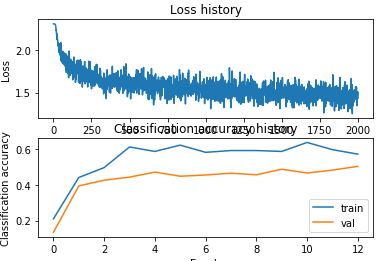
\includegraphics[width=\textwidth]{img/Img_1.JPG}
         \caption{It=2000, Batch Size=300}
         \label{Iteration=2000, Batch Size=300}
     \end{subfigure}
     \hfill
     \begin{subfigure}[b]{0.2\textwidth}
         \centering
         \includegraphics[width=\textwidth]{img/Img_2.JPG}
         \caption{It=3000, Batch Size=300}
         \label{fig:three sin x}
     \end{subfigure}
     \hfill
     \begin{subfigure}[b]{0.2\textwidth}
         \centering
         \includegraphics[width=\textwidth]{img/Img_3.JPG}
         \caption{It=3000, Batch Size=200}
     \end{subfigure}
     \hfill
     \begin{subfigure}[b]{0.2\textwidth}
         \centering
         \includegraphics[width=\textwidth]{img/Img_4.JPG}
         \caption{It=4000, Batch Size=200}
     \end{subfigure}
      \hfill
     \begin{subfigure}[b]{0.2\textwidth}
         \centering
         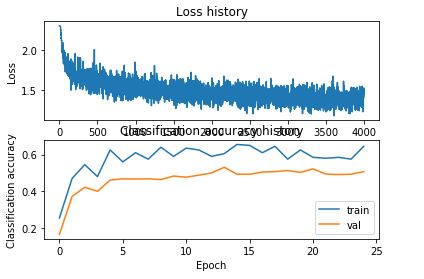
\includegraphics[width=\textwidth]{img/img_5.JPG}
         \caption{It=4000, Batch Size=300}
     \end{subfigure}
      \hfill
     \begin{subfigure}[b]{0.2\textwidth}
         \centering
         \includegraphics[width=\textwidth]{img/Img_6.JPG}
         \caption{It=5000, Batch Size=300}
     \end{subfigure}
      \hfill
     \begin{subfigure}[b]{0.2\textwidth}
         \centering
         \includegraphics[width=\textwidth]{img/Img_7.JPG}
         \caption{It=5000, Batch Size=200}
     \end{subfigure}
      \hfill
     \begin{subfigure}[b]{0.2\textwidth}
         \centering
         \includegraphics[width=\textwidth]{img/Img_8.JPG}
         \caption{It=5000, Batch Size=100}
     \end{subfigure}
     \hfill
     \begin{subfigure}[b]{0.2\textwidth}
         \centering
         \includegraphics[width=\textwidth]{img/Img_9.JPG}
         \caption{It=6000, Batch Size=300}
     \end{subfigure}
     \hfill
     \begin{subfigure}[b]{0.2\textwidth}
         \centering
         \includegraphics[width=\textwidth]{img/Img_10.JPG}
         \caption{It=6000, Batch Size=200}
     \end{subfigure}
      \hfill
     \begin{subfigure}[b]{0.2\textwidth}
         \centering
         \includegraphics[width=\textwidth]{img/Img_11.JPG}
         \caption{It=6000, Batch Size=500}
     \end{subfigure}
      \hfill
     \begin{subfigure}[b]{0.2\textwidth}
         \centering
         \includegraphics[width=\textwidth]{img/Img_12.JPG}
         \caption{It=6000, Batch Size=100}
     \end{subfigure}
        \caption{Loss and Train/ Validation accuracies}
        \label{fig:three graphs}
\end{figure}
\newpage
\section*{Question 4 - Multi-layer perceptron using PyTorch}
\section* {4. c}

\begin{table}[ht]
\begin{center}
\caption{Train and Test Accuracy for multiple layers.}
\begin{tabular}{rrlll}
\toprule
 Total Layers &  Epochs & Hidden Layer Size & Train Accuracy & Test Accuracy \\
\midrule
            3 &      20 &            250,\ 50 &         55.3 \% &        56.8 \% \\
            2 &      20 &               100 &         55.8 \% &        54.0 \% \\
            3 &      10 &            250,\ 50 &         53.4 \% &        53.1 \% \\
            2 &      10 &               100 &         52.2 \% &        51.5 \% \\
            5 &      20 &   200,\ 200,\ 250,\ 150 &          9.8 \% &        10.0 \% \\
            4 &      10 &       150,\ 100,\ 200 &          9.8 \% &         9.0 \% \\
            4 &      20 &       150,\ 100,\ 200 &          9.8 \% &         9.0 \% \\
            5 &      10 &   200,\ 200,\ 250,150 &          9.8 \% &         9.0 \% \\
\bottomrule
\end{tabular}
\end{center}
\end{table}

In table 1 we can see that for all tests with a number of layers greater than 3, the accuracy obtained is less than 10\%. The best accuracies were obtained in networks with 2 and 3 layers where the number of epochs was equal to 20. In particular, the best result among those tested was obtained by setting 2 hidden layers with number of neurons of 250 and 50 respectively, and a number of epochs equal to 20.









%------------------------------------------------
\end{document}
